\subsection{\textcolor{magenta}{Préparer le laser}}
\begin{center} $\ast\ast\ast$ Si le laser est déjà en Standby, passer tout de suite à la section \ref{ssec:allumer_le_laser}. $\ast\ast\ast$ \end{center}
\begin{enumerate}
    \item À l'arrière du \textit{contrôleur Verdi} (voir figure~\ref{fig:controleur-verdi}, mettre l'interrupteur sur \textit{On}).
        \begin{figure}[H]
        \centering
        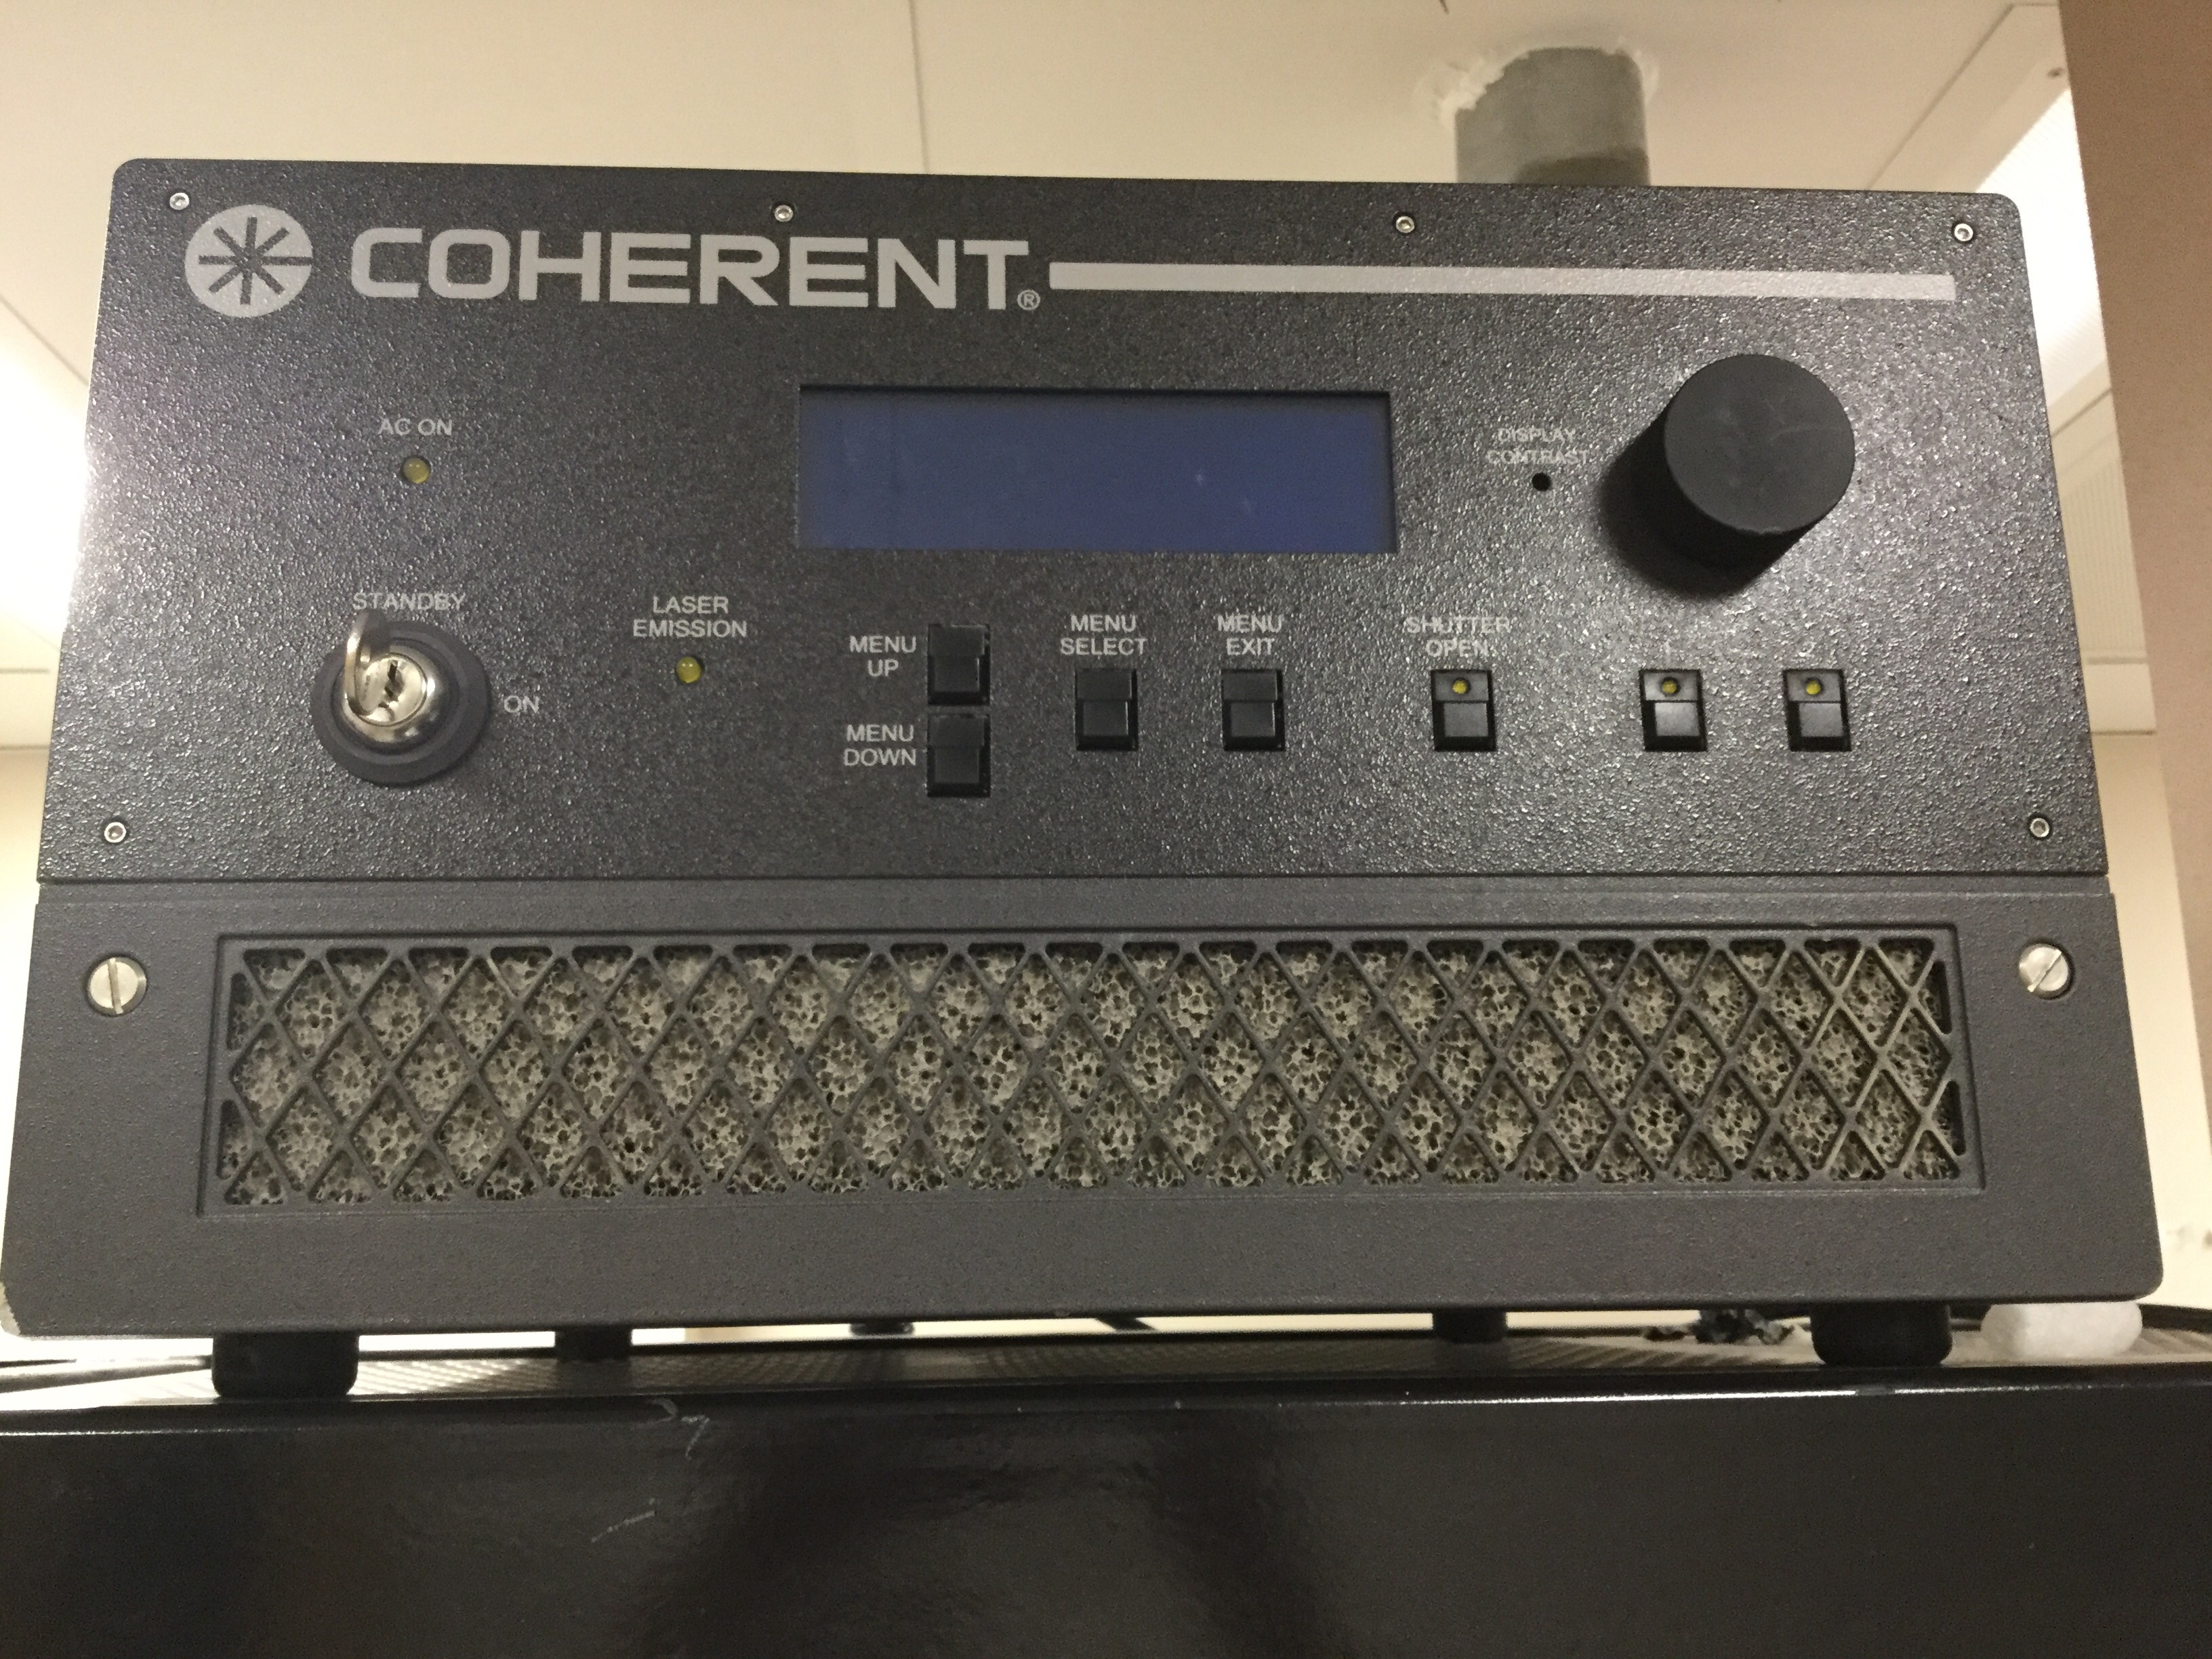
\includegraphics[width=12cm]{controleur-verdi.jpg}
        \caption{Contrôleur du \textit{Verdi}}
        \label{fig:controleur-verdi}
        \end{figure}
    \item Sur chaque refroidisseur (voir figure~\ref{fig:cooler}, peser sur le bouton \textit{Run/Standby}. Le message \textit{Standby Mode} devrait être remplacé par la valeur de la température.
        \begin{figure}[H]
        \centering
        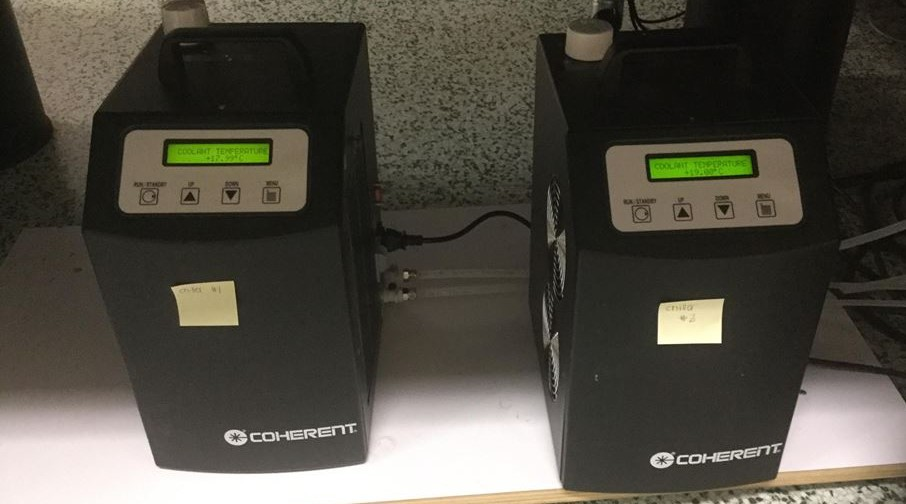
\includegraphics[width=10cm]{cooler.jpg}
        \caption{Refroidisseurs: l'un contrôle le \textit{Verdi}, l'autre le \textit{Mira} et le \textit{RegA}}
        \label{fig:cooler}
        \end{figure}
    \item Peser sur le bouton \textit{Menu/Select}. À l'aide des boutons \textit{Menu Up} et \textit{Menu Down}, aller dans ???. À l'aide de la roulette, ajuster le puissance à 17~W. vérifier que le \textit{'LBO'} est sur \textit{'heating'}. 
    \item Revenir à l'accueil avec le bouton \textit{Menu Exit}. Attendre que la puissance affichée se stabilise à 17~W.
\end{enumerate}